\documentclass[aps, prl, twocolumn, longbibliography, linenumbers, superscriptaddress]{revtex4-2}

\usepackage{amsmath} 
\usepackage{amssymb}
\usepackage{amsthm} 
\usepackage{graphicx} 
\usepackage{color}
\newcommand{\blue}{\color{blue}}
\newcommand{\red}{\color{red}}
%\usepackage{hyperref} 
\usepackage{float}

\newcommand{\vect}[1]{\mathbf{#1}}

\begin{document}

\title{Subdiffusive random growth of bacterial size}

\author{Jialiang Wei}
\affiliation{School of Physics, Peking University, Beijing, China}
\author{Yichen Yan}
\affiliation{Center for Quantitative Biology, Peking University, Beijing, China}
\affiliation{Peking-Tsinghua Center for Life Sciences, Peking University, Beijing, China}
\author{Jie Lin}
\email{linjie@pku.edu.cn}
\affiliation{Center for Quantitative Biology, Peking University, Beijing, China}
\affiliation{Peking-Tsinghua Center for Life Sciences, Peking University, Beijing, China}
\date{\today}
\begin{abstract}
While the regulation of bacterial cell size has been widely studied across generations, the stochastic nature of cell volume growth remains elusive within the cell cycle. Here, we investigate fluctuations in cell volume growth and report subdiffusive random growth. Specifically, the mean square displacement of the logarithmic volume scales as $\Delta t^\alpha$ with an exponent $\alpha \approx 0.25$. This low exponent implies negative temporal correlations in growth rate noise on timescales of minutes, which are significantly faster than those of gene expression dynamics. We attribute this phenomenon to the physical mechanics of the cell wall. By modeling the cell wall as a complex viscoelastic material with power-law-distributed relaxation times, we successfully reproduce the observed subdiffusive behavior. Our results suggest that heterogeneous cell-wall viscoelasticity governs short-timescale fluctuations in bacterial growth rate, leading to more accurate doubling-time regulation.
\end{abstract}
\maketitle

{\it Introduction---}Understanding how bacteria regulate their size is a fundamental question in quantitative biology \cite{Ho2018modeling, Cadart2019physics}. Phenomenological models, such as the ``adder'' model, have successfully described cell size control at the intergenerational level \cite{Amir2014cell, Campos2014constant, Taheri2015cell}. Regarding the average growth dynamics within a cell cycle, it has been suggested that bacterial cell volumes grow exponentially over time \cite{Wang2010robust, Godin2010using, Campos2014constant, Taheri2015cell}. Nevertheless, recent studies on {\it Escherichia coli} and {\it Caulobacter crescentus} have suggested that growth is not strictly exponential but exhibits a ``superexponential'' acceleration toward the end of the cell cycle \cite{Kar2021distinguishing, Cylke2023super, Cylke2025gene}. Meanwhile, what is even more elusive is the stochastic nature of cell volume growth on top of the deterministic growth, and how a bacterial cell regulates its volume on a shorter time scale than the cell cycle.

In this Letter, we first employ a minimal drifted Brownian model where the growth-rate noise is modeled as white noise. We find that, given the same growth-rate noise magnitude as the experimental data, the resulting doubling-time distribution exhibits a much larger CV (coefficient of variation) than the experimental data, suggesting that the experimental growth-rate noise is colored. We then directly investigate the fluctuations of cell volume growth, and indeed, we observe that the random growth rate of cell volume exhibits a subdiffusive fluctuation. Suppose we consider the growth rate as the velocity of an imaginary particle and the logarithmic volume $x \equiv \ln(V/\bar{V}_b)$ as the particle position; the mean square displacement (MSD) of $x$ scales as $\sigma^2_x (\Delta t) \sim \Delta t^{\alpha}$ with an exponent $\alpha \approx 0.25$ that is smaller than one. This subdiffusion implies that the growth rate noise exhibits negative temporal correlations.

Given that the subdiffusion occurs on a time scale of minutes, much shorter than the time scales of significant changes in protein concentrations \cite{Kiviet2014stochasticity, Milo2015cell}, we hypothesize that this phenomenon has a physical origin. Given the fact that the deformation of the cell wall is a prerequisite for cell volume growth, we propose that the subdiffusive random growth of cell volume is a consequence of the mechanical properties of the cell wall \cite{Seltmann2002bacterial, Meroueh2006three, Rodriguez2008surface, Auer2017bacterial, Weber2022power}. Specifically, we model the cell wall as a complex viscoelastic material composed of multiple serially connected Voigt elements, where each element is a parallel connection of a purely viscous dashpot and purely elastic spring. We assume the relaxation times of the elements are random and follow a power-law distribution. This simple model successfully reproduces subdiffusive growth behavior, and our results suggest that the viscoelastic and heterogeneous cell wall fundamentally constrains bacterial growth. Importantly, the subdiffusive random noise in bacterial growth rate helps cells to achieve a more accurate regulation of doubling-time distribution.

\begin{figure}[hbt!]
	\centering
	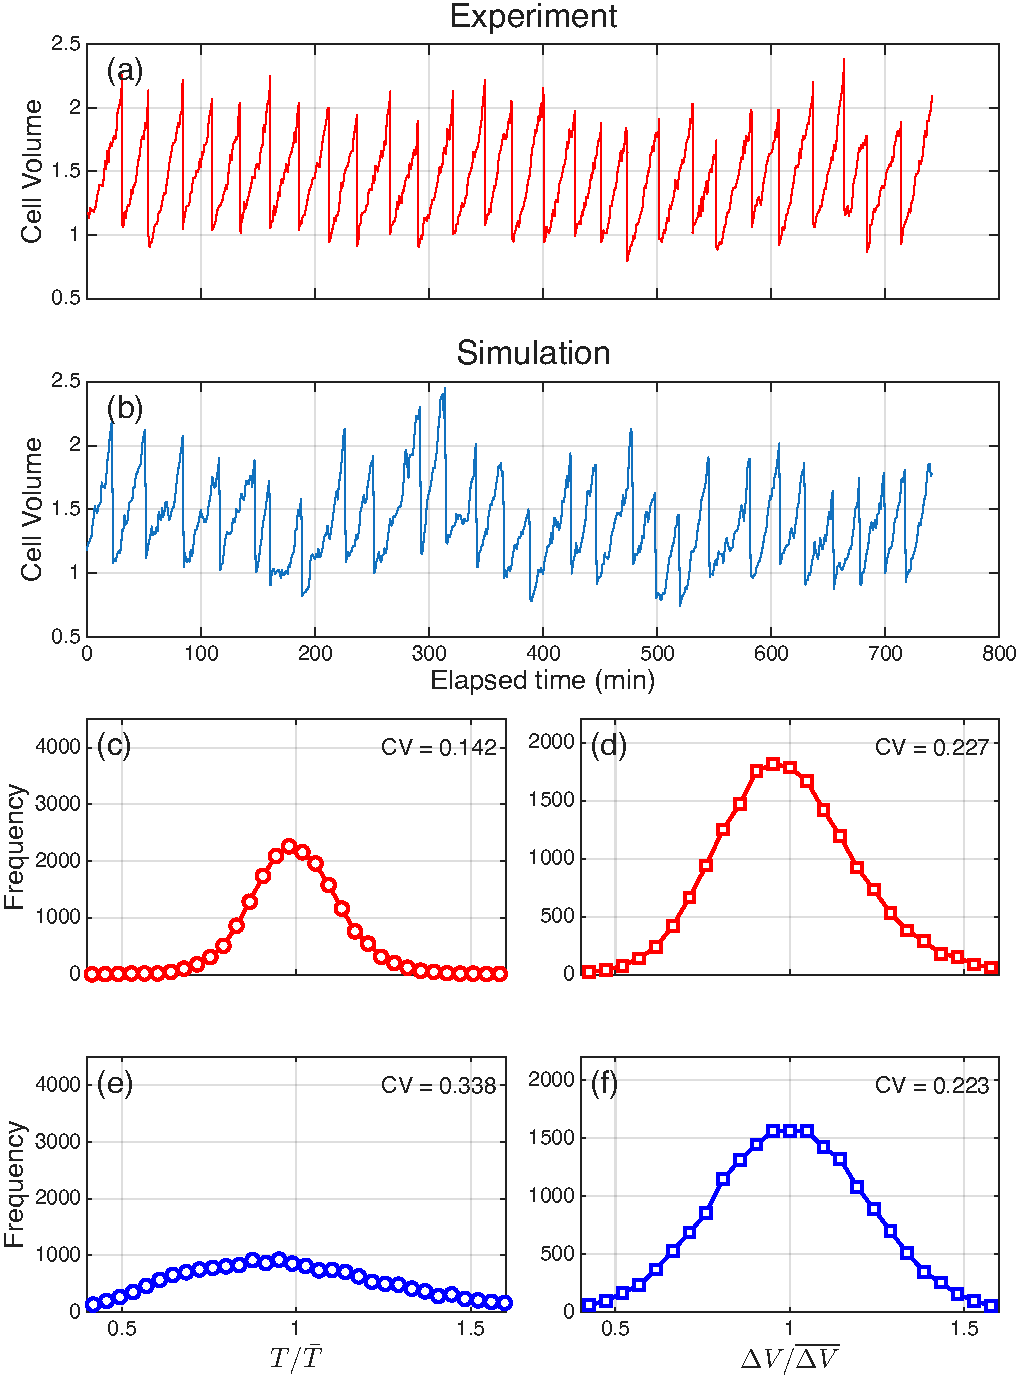
\includegraphics[width=0.48\textwidth]{traj.pdf}
	\caption{Comparison of cell cycle dynamics between experimental data and the null model. (a) Cell volume vs. time for the experimental data of {\it E. coli} in the glucose+12 a.a. medium in Ref. \cite{Taheri2015cell}, where the cell volume is normalized by the average birth volume $\bar V_b$. (b) The same as (a) but for the simulation data. Here, $a=0.026$, $b=0.037$, with the time unit 1 min. (c-d) Experimental distributions of the normalized doubling time $T/\overline{T}$ (c) and normalized added volume throughout one cell cycle $\Delta V/\overline{\Delta V}$ (d). (e-f) The corresponding distributions generated by the null model simulation.}
	\label{fig:traj}
\end{figure}

\begin{figure*}[hbt!]
	\centering
	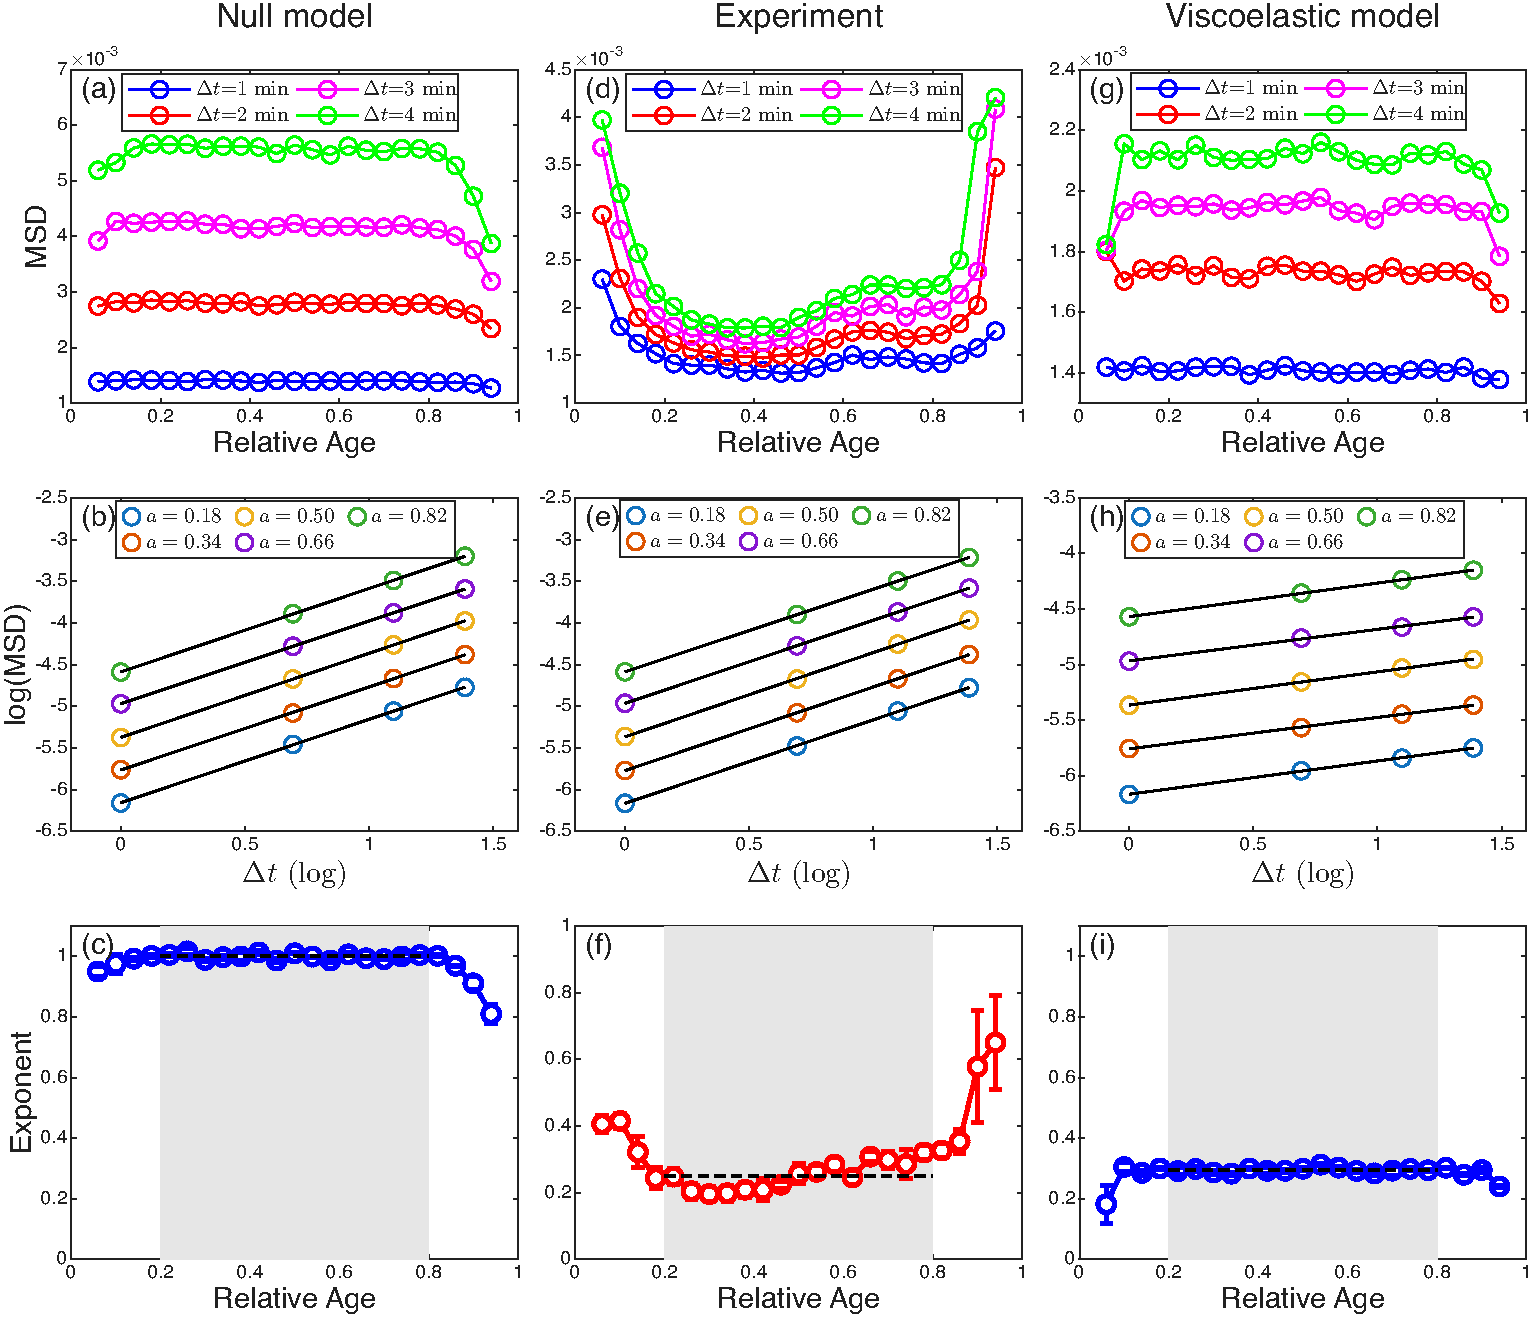
\includegraphics[width=0.9\textwidth]{fluctuation.pdf}
	\caption{Subdiffusive random growth of cell volume. (a) $\sigma^{2}_x (\Delta t)$ vs. the relative age for time intervals $\Delta t = 1, 2, 3,$ and $4$ min for the simulation data of the null model. (b)  $\sigma^{2}_x (\Delta t)$ vs. $\Delta t$ for several relative ages, from which we calculated the diffusion exponent. Curves for different relative ages are vertically shifted for visual clarity to highlight the robust power-law scaling. (c) The diffusion exponent ($\alpha$) calculated from the simulation data as a function of the relative age, showing the reliable regime where $\alpha$ equals the ground truth $1$. (d-f) The same analysis as (a-c) but for the same experimental data of {\it E. coli} in Fig.~\ref{fig:traj}(a). (g-i) The same as (a-c) but for the viscoelastic model. The dashed line in (c, f, i) is the average exponent in the reliable regime.}
	\label{fig:fluctuation}
\end{figure*}

{\it The null model of stochastic cell growth---}We introduce a minimal model of cell volume growth as a control for the experimental data and define $x\equiv \ln(V/\bar V_b)$, where $V$ is the cell volume and $\bar V_b$ is the birth volume averaged over cell cycles, which is a constant. In the minimal model, $x$ follows a drifted Brownian motion:
\begin{equation}
	\mathrm{d}x = a \mathrm{d}t + b \mathrm{d}W.
	\label{eq:GBM}
\end{equation}
Here, $t$ is time, $a$ is the deterministic growth rate, and $b$ is the noise intensity. $\mathrm{d}W$ represents a Wiener process increment, which is a Gaussian-distributed random number with mean equal to zero and variance equal to $\mathrm{d}t$ \cite{Gardiner2004handbook}. Cell division is implemented using the adder model \cite{Amir2014cell, Taheri2015cell, Ho2018modeling}: $V_d(n)=V_b(n)+V_0 + \zeta $ and $V_b(n+1)=V_d(n)/2$. Here, $n$ is the generation number, $V_d$ is the division volume, $V_b$ is the birth volume, $V_0$ is a constant, and $\zeta$ is a Gaussian-distributed random variable.

We remark that this null model of stochastic random growth has several advantages. First, it is presumably the simplest model for describing an exponentially growing cell volume, given its constant noise magnitude $b$. More importantly, it is consistent with the experimental data, in which we find an approximately constant variance of $\Delta x$ over most of the cell cycle. Therefore, we assume a constant noise magnitude in Eq. (\ref{eq:GBM}) instead of assuming an $x$-dependent noise magnitude as in other models \cite{Biswas2014scaling}. We note that even if we assume an $x$-dependent noise magnitude, our conclusions regarding the null model remain the same (Fig.~S5).
	
We simulate the null model and compare the simulation results with the experimental data (Fig.~\ref{fig:traj}). To make a meaningful comparison, we set the noise magnitude $b$ such that the variances of $\Delta x$ during 1 min are approximately the same between the simulation and experiment (one can see this by comparing Fig.~\ref{fig:fluctuation}(a, g) and Fig.~\ref{fig:fluctuation}(d), which we introduce later). In the meantime, we also ensure that the white-noise null model has similar statistics for the total volume increment over a cell cycle by choosing appropriate parameters for the adder model [Fig.~\ref{fig:traj}(d, f)]. Surprisingly, we find that, given these constraints on the simulation parameters, the resulting doubling-time distribution shows a much larger CV (coefficient of variation) than that of the experiment [Fig.~\ref{fig:traj}(c, e)]. This observation indicates that the noise term in Eq. (\ref{eq:GBM}) should be colored rather than white; more specifically, the noise should be anti-correlated in time, and its accumulation should exhibit subdiffusion. In the following, we compute the variance of $\Delta x$ and show that this is indeed the case.

{\it Subdiffusive random growth---}Bacterial cell volume is well regulated across cell cycles; however, it is still elusive whether cell volume growth is regulated on a shorter time scale. Therefore, we study fluctuations in cell volume growth using the minimal model as a control. We calculate $\sigma_x^2(\Delta t)= \langle \Delta x(\Delta t)^2\rangle- \langle \Delta x(\Delta t)\rangle^2$ where $\Delta x(\Delta t)= x(t+\Delta t)-x(t)$ given a time interval $\Delta t$; here, the average is over cell cycles conditioned on a given relative age, which we call the mean square displacement (MSD) of $x$ in the following. For the minimal model, $x$ is a random walk with a constant drift; therefore, $\sigma^2_x(\Delta t) \sim \Delta t$ [Fig.~\ref{fig:fluctuation}(a-c)]. Indeed, the measured exponent was close to one as long as the relative age is not close to zero or one [Fig.~\ref{fig:fluctuation}(b, c)], from which we introduce a regime where the measured exponent is reliable (the shaded area in Fig.~\ref{fig:fluctuation}(c)). Strikingly, we find that the experimental data of $x$ implements a subdiffusive noise [Fig.~\ref{fig:fluctuation}(d-f)]:
\begin{equation}
	\sigma^2_x (\Delta t) \sim \Delta t^{\alpha}.
	\label{eq:anomalous_exponenMukherjee2025bacterialt}
\end{equation}
Notably, $\sigma^2_x(\Delta t)$ in the experimental data is significantly larger at the early and late stages of the cell cycle [Fig.~\ref{fig:fluctuation}(d)], which may be generated by the morphological rearrangements during cell birth and division. Intriguingly, the $\alpha$ exponent changes mildly throughout the cell cycle, with an average value $\alpha\approx 0.25$ in the reliable regime. We also analyze the MSD using growth rate data derived from cell length and surface area and find similar subdiffusive behavior (Fig.~S6). More importantly, this subdiffusive scaling is robust across a wide range of growth rates and nutrient conditions (Fig.~S7).  We further confirm the subdiffusion by computing the autocorrelation of the discrete growth-rate noise and obtain a consistent negative correlation (Fig.~S8). Furthermore, this subdiffusive exponent $\alpha$ can also be robustly extracted by computing the MSD conditioned on the absolute elapsed time (Fig.~S9).


\begin{figure}[htb!]
	\centering
	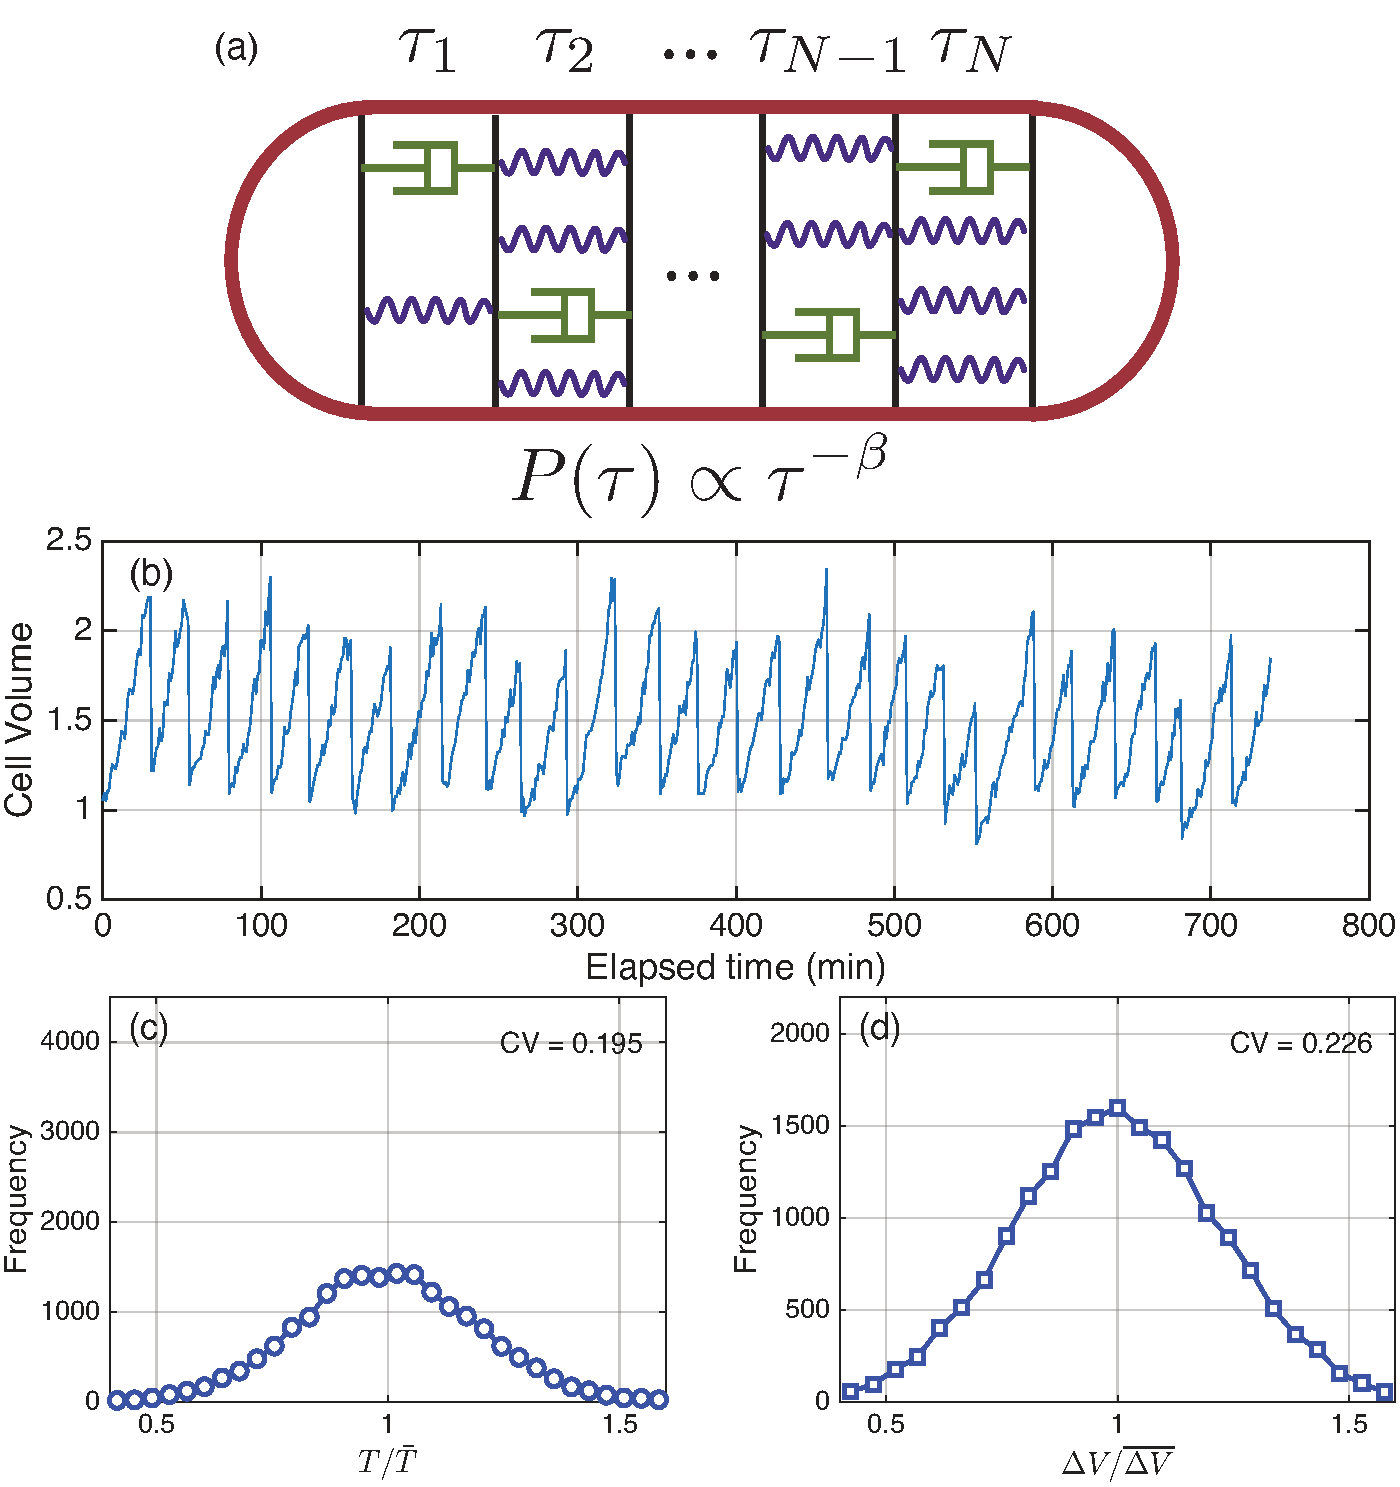
\includegraphics[width=0.48\textwidth]{voigt.pdf}
	\caption{The viscoelastic model of the cell wall reproduces the subdiffusive random growth. (a) We model the cell wall as a serial connection of multiple Voigt elements, each with an elastic component (the spring) and a viscous component (the dashpot). We assume that the relaxation time of each element is random due to the random elastic constant, such that the relaxation time follows a power-law distribution. (b) The same as Fig.~\ref{fig:traj}(a), but we replace the white noise with the colored noise $\xi(t)$ generated by the random Voigt model. (c-d) Distributions of the normalized doubling time $T/\overline{T}$ (c) and normalized added volume throughout one cell cycle $\Delta V/\overline{\Delta V}$ (d) generated by the viscoelastic model simulation. In (b-d) and Fig.~\ref{fig:fluctuation}(g-i), we set the dimensionless noise strength $A_{\sigma} \approx 3.2 \times 10^{-2}$ so that the simulated $\sigma_x^2$ at $\Delta t=1$ min is approximately the same as in the experiments. $\tau_0 = 0.001$,} the deterministic growth rate $a=0.026$, and $N=2371$.
	\label{fig:voigt}
\end{figure}

{\it Modeling cell-volume dynamics as a complex viscoelastic material---}Because the subdiffusion occurs on a time scale of minutes [Fig.~\ref{fig:fluctuation}(e)], it is unlikely to be generated by activities associated with gene expression, which usually takes a doubling time for the protein concentrations to change significantly in bacteria \cite{Kiviet2014stochasticity, Milo2015cell}. Therefore, we hypothesize that the subdiffusion comes from a physical process. Considering that cell volume growth always accompanies cell wall growth, and that the cell wall is a complex viscoelastic material \cite{Rodriguez2008surface, Weber2022power, Mukherjee2025bacterial}, we propose that the cell wall mediates the subdiffusive random growth.

We introduce the viscoelastic model of cell-wall mechanics in which we model the cell wall, a peptidoglycan network, as a serial connection of $N$ Voigt elements [Fig.~\ref{fig:voigt}(a)], which allows us to unify long-term growth and short-term subdiffusion. Specifically, we decompose the total strain of the cell wall as $x=x_0 + \sum_{i=1}^N x_i/N$, which satisfies
\begin{equation}
	\begin{aligned}
	&\eta_0 \frac{dx_0}{dt} = \sigma,\\
	&\eta \frac{dx_i}{dt} = -E_i x_i + \sigma.
	\end{aligned}
\end{equation}
Here, $x_0$ is the growth strain representing the cell wall elongation resulting from cleavage of peptide bonds. This process can be effectively modeled as a growth dashpot ($\eta_0$) connected in series. $x_i$ is the strain of the Voigt elements, and we assume that the overall strain contributed by the Voigt elements is the average over them.
	
One should note that the growth viscosity $\eta_0$ is an effective viscosity set by the time scale of cell-wall cleavage mediated by endopeptidases \cite{Mukherjee2025bacterial}. Meanwhile, the micro-viscosity $\eta$ and the elastic modulus $E_i$ are material properties independent of cell growth. Here, $\sigma$ is the cell wall tension, which is generated by the turgor pressure $P$ (i.e., the difference between cytoplasmic and external osmotic pressures) \cite{Arnoldi2000bacterial, Deng2011direct, Rojas2014response, Zhang2021measurement, Ye2025physical}. $\sigma$ is related to $P$ via $\sigma = rP/2d$, where $r$ is the cell width and $d$ is the cell wall thickness. In the limit $\eta\rightarrow 0$, our model reduces to the Maxwell model of cell-wall mechanics introduced by Mukherjee et al., where the effective elastic modulus $1/E_{\rm{eff}}= (1/N)\sum_{i=1}^{N}1/E_i$ \cite{Mukherjee2025bacterial}.

We assume that the subdiffusion comes from the fluctuating cell wall tension, which can be decomposed as $\sigma=\bar{\sigma}+\delta \sigma(t)$. Here, $\bar{\sigma}$ is a constant and $\delta\sigma(t)$ is the fluctuating part, which we model as white noise with the autocorrelation function, $\langle \delta \sigma(t_1)\delta \sigma(t_2)\rangle = 2A_\sigma \delta(t_1-t_2)$, where $A_{\sigma}$ is a constant. Decomposing the strain as a sum of a deterministic and a stochastic part, $x_i=\bar{x}_i +\xi_i$, we obtain the dynamics of $\xi_i$ as
\begin{equation}
	\eta \frac{\mathrm{d} \xi_i}{\mathrm{d}t} = -E_i \xi_i + \delta \sigma.
	\label{eq:constitutive}
\end{equation}
Under normal conditions, the system relaxes to equilibrium where the deterministic strain vanishes ($\bar{x}_i = 0$), leaving $x_i$ driven purely by the stochastic stress fluctuations $\delta \sigma$.
Finally, the dynamics of the total strain can be formally written as
\begin{equation}
	\mathrm{d}x = a \mathrm{d}t + \mathrm{d} \xi(t), 
	\label{voigt_xt}
\end{equation}
where $a = \bar{\sigma}/\eta_0$ is the deterministic growth rate, which we take to be constant for simplicity, and $\xi(t) = \sum_i \xi_i(t)/N$.
Note that we neglect the stochastic component of the growth strain $x_0$ because it follows $\eta_0  d\xi_0/dt=\delta \sigma$, yielding only normal diffusion, which is irrelevant to the subdiffusion we seek to understand.


In the following, we non-dimensionalize the model by setting the time unit $t_0=1$ min, the stress unit as $\eta/t_0$, and all variables are dimensionless unless otherwise mentioned. From Eq.~(\ref{eq:constitutive}), we introduce the relaxation time as $\tau_i = \eta/E_i$ for each Voigt element, which we model as a random variable and which follows a power-law distribution [Fig.~\ref{fig:voigt}(a)]:
\begin{equation}
	P(\tau)=C\tau^{-\beta},
	\label{eq:power-law-P-tau}
\end{equation}
with a lower bound $\tau_0$ and the normalization factor $C=(\beta-1)\tau_0^{\beta-1}$. Solving Eq.~(\ref{eq:constitutive}) for a specific element yields
\begin{equation}
	 \xi_i(t) = \int_{-\infty}^{t} e^{-\frac{t-t'}{\tau_i}} \delta \sigma(t') \mathrm{d}t'.
	\label{eq:gamma_tau_integral_en}
\end{equation}
Taking account of the randomly distributed relaxation time, the overall cell growth noise $\xi(t)$ becomes
\begin{equation}
	\xi(t)  = C \int_{0}^{\infty} g^{1-\beta} F(g/\tau_0) \delta \sigma(t-g) \mathrm{d}g,
	\label{eq:gamma_kernel_en}
\end{equation}
where $F(x)=\int_0^{x} v^{\beta-2} e^{-v}\mathrm{d}v \equiv \gamma(\beta-1, x)$ is the lower incomplete gamma function. Given Eq.~(\ref{eq:gamma_kernel_en}), we find the MSD of $x(t)$ (Supplemental Material (SM) Section IV) as
\begin{equation}
	\begin{aligned} 
		 \sigma_x^2(\Delta t) &= \langle [\xi(\Delta t)-\xi(0)]^2\rangle \\
		&= 4C^2 A_{\sigma} \Delta t^{3-2\beta} \int_{0}^{\infty} u^{2\beta -4}\Big[F\Big(\frac{\Delta t}{u\tau_0}\Big)^2\\
		&\quad - (1+u)^{1-\beta} F\Big(\frac{\Delta t}{u\tau_0}\Big) F\Big(\frac{\Delta t}{u\tau_0}+\frac{\Delta t}{\tau_0}\Big) \Big] \mathrm{d}u.
	\end{aligned}\label{msd}
\end{equation}
We find that in the limit $\Delta t/\tau_0 \gg 1$, with the condition $1<\beta <3/2$, the integral in Eq. (\ref{msd}) is a finite constant (see detailed derivation in SM Section IV). Consistently, we obtain $\alpha = 3 - 2\beta$ and infer $\beta= 1.375$ from the measured $\alpha$ exponent [Fig.~\ref{fig:fluctuation}(f)].

To confirm whether the random Voigt model can reproduce the experimental phenomena, we simulate the minimal model Eq.~(\ref{voigt_xt}) with cell cycles included [Fig.~\ref{fig:voigt}(b)], similar to the simulations in Fig.~\ref{fig:traj}. We explicitly generate the noise $\xi(t)$ by simulating $N=2371$ Voigt elements, whose relaxation times are sampled from Eq.~(\ref{eq:power-law-P-tau}) with $\tau_0=0.001$. We set $\beta=1.375$ so that the predicted subdiffusive exponent for the MSD of logarithmic volume is $\alpha=0.25$. By averaging $\xi_i$ over all elements, we obtain the time-dependent noise $\xi(t)$ in Eq.~(\ref{voigt_xt}) (End Matter). Notably, the incorporation of colored noise significantly narrows the distribution of doubling time [Fig.~\ref{fig:voigt}(c)], with a CV much closer to that of the experimental doubling-time distribution, compared with the null model given the same MSD at 1 min [Fig.~\ref{fig:traj}(c, e)]. More importantly, the viscoelastic model successfully reproduces the subdiffusive random growth of bacterial cell volume [Fig.~\ref{fig:fluctuation}(g-i)].

We note that our simulation results are insensitive to the maximum values of the relaxation-time distribution, which scales as $\tau_{\max}\sim \tau_0 N^{1/(\beta-1)}$, since they are much longer than the time scale of the subdiffusion we observe here. Indeed, the simulation results based on different $N$ values yield essentially identical results [Fig. S11(b)]. To verify whether the measured exponent approaches the predicted value in the limit of $\Delta t/\tau_0\gg 1$, we change $\tau_0$ (with $A_{\sigma}$ and $N$ changing correspondingly to ensure the prefactor of the long-term subdiffusion and the expected maximum relaxation time remain invariant). Indeed, the measured exponent approaches the predicted value $\alpha=0.25$ as $\tau_0$ decreases [Fig.~S10(a)]. We also simulate an extended model in which the deterministic growth rate in each cell cycle is random, with the noise intensity chosen to match the experimental data; we confirm that the subdiffusive nature is robust against fluctuations in the deterministic growth rate (Fig.~S11).

{\it Discussion---}In this work, we demonstrate that the stochastic growth of bacterial cell volume exhibits subdiffusive fluctuations, a phenomenon that cannot be accounted for by white-noise growth models. The subdiffusion with an exponent $\alpha \approx 0.25$ suggests that negative temporal correlations govern growth fluctuations. This ``memory'' in the growth process occurs on the scale of minutes, which is significantly shorter than the time scale of growth rate noise generated by biochemical processes—such as gene expression, protein synthesis, or cellular metabolism—that operate on the scale of hours or a doubling time \cite{Kiviet2014stochasticity}. Instead, our analysis of experimental data points toward a mechanical origin by treating the cell wall as a complex viscoelastic material. The broad distribution of cell wall relaxation times implies significant heterogeneity within the peptidoglycan network, potentially stemming from the stochastic nature of crosslink density and local architectural disorder. Our finding relates the subdiffusive exponent $\alpha$ governing the macroscopic growth to the relaxation-time distribution exponent $\beta$ governing the microscopic material properties. Our work suggests that the peptidoglycan network is a complex material whose multi-scale relaxation dynamics fundamentally constrain the stochastic nature of cell growth and help cells maintain a narrower distribution of doubling time. We have also analyzed the impact of various experimental perturbations as implemented in Ref. \cite{Mukherjee2025bacterial} on the prefactor and the scaling exponent of the subdiffusion (SM Section III).

Beyond bacterial growth, our study also highlights the need for rigorous null models when analyzing biological data. Previous works have shown that the growth rate $a$ was not constant during the cell cycle for {\it E. coli} and other bacteria \cite{Kar2021distinguishing, Cylke2023super, Cylke2025gene}. Interestingly, even the minimal null model with a strictly constant growth rate can exhibit apparent growth acceleration or deceleration. Specifically, conditioning the average growth rates on relative age, volume, or elapsed time inherently introduces systematic biases, which may or may not be eliminated by taking the time window between two successive measurements to zero (SM Section I).

\begin{acknowledgments}
	We thank Poyi Ho and Ziming Zhao for helpful discussions related to this work. The research was funded by the National Key Research and Development Program of China (2024YFA0919600) and supported by Peking-Tsinghua Center for Life Sciences grants.
\end{acknowledgments}

\bibliography{Lin_Dec_05_2025}

\subsection{End Matter}
\subsubsection{Details of numerical simulations}
We perform numerical simulations of the stochastic growth dynamics using a multi-scale integration scheme. The stochastic differential equation (SDE) for cell volume growth [Eq.~(\ref{eq:GBM})] is integrated with a time step of $ 0.05$ min. To match the 1-min sampling interval of the experimental data \cite{Taheri2015cell}, we sample the simulation trajectories every 20th data point. The division process follows the adder model, with noise magnitudes in both the SDE and the division volume tuned to reproduce the observed volume trajectories in experiments.

For the viscoelastic growth model (Fig.~\ref{fig:voigt}), we generate the colored noise $\xi(t)$ by simulating $N=2371$ Voigt elements with a time step of $0.001$ min when $\tau_0 = 0.001$. The SDE for cell volume growth [Eq.~(\ref{voigt_xt})] is integrated with a time step of $0.05$ min. To ensure the colored noise statistics reach a stationary state, we implement a ``pre-warming'' period for each lineage in which the viscoelastic model is equilibrated for 10 min before being coupled to the volume SDE. The colored noise $\xi(t)$ is generated independently for each simulated lineage. Specifically, we simulate $394$ independent lineages, each spanning $47$--$48$ consecutive cell cycles (totaling $18,524$ cell cycles) to match experimental statistics. For each lineage, the set of relaxation times $\{\tau_i\}$ for the $N$ Voigt elements is randomly sampled once and held fixed throughout all generations. Furthermore, within a given lineage, the internal viscoelastic states—and consequently the colored noise $\xi(t)$—are continuously inherited across cell divisions from one generation to the next without resetting.

Note that given $N$ Voigt elements, the maximum relaxation time scales as $\tau_{\max}\sim \tau_0 N^{1/(\beta-1)}$. In Fig.~S10, we change $\tau_0$, and in the meantime, change $A_{\sigma}$ as $A_{\sigma}(\tau_0)=A_{\sigma}(\tau_0=0.001) (\tau_0/0.001)^{2-2\beta}$ and $N(\tau_0)=N(\tau_0=0.001) (\tau_0/0.001)^{1-\beta}$ to ensure the prefactor of the MSD [Eq.~(\ref{msd})] and the maximum relaxation time remain invariant.

\end{document}
